\documentclass[11pt,]{article}
\usepackage{lmodern}
\usepackage{amssymb,amsmath}
\usepackage{ifxetex,ifluatex}
\usepackage{fixltx2e} % provides \textsubscript
\ifnum 0\ifxetex 1\fi\ifluatex 1\fi=0 % if pdftex
  \usepackage[T1]{fontenc}
  \usepackage[utf8]{inputenc}
\else % if luatex or xelatex
  \ifxetex
    \usepackage{mathspec}
  \else
    \usepackage{fontspec}
  \fi
  \defaultfontfeatures{Ligatures=TeX,Scale=MatchLowercase}
\fi
% use upquote if available, for straight quotes in verbatim environments
\IfFileExists{upquote.sty}{\usepackage{upquote}}{}
% use microtype if available
\IfFileExists{microtype.sty}{%
\usepackage{microtype}
\UseMicrotypeSet[protrusion]{basicmath} % disable protrusion for tt fonts
}{}
\usepackage[margin = 1.5in]{geometry}
\usepackage{hyperref}
\PassOptionsToPackage{usenames,dvipsnames}{color} % color is loaded by hyperref
\hypersetup{unicode=true,
            pdftitle={ARMA GARCH Processes},
            pdfauthor={Abhinav Anand, IIMB},
            colorlinks=true,
            linkcolor=blue,
            citecolor=magenta,
            urlcolor=red,
            breaklinks=true}
\urlstyle{same}  % don't use monospace font for urls
\usepackage{color}
\usepackage{fancyvrb}
\newcommand{\VerbBar}{|}
\newcommand{\VERB}{\Verb[commandchars=\\\{\}]}
\DefineVerbatimEnvironment{Highlighting}{Verbatim}{commandchars=\\\{\}}
% Add ',fontsize=\small' for more characters per line
\usepackage{framed}
\definecolor{shadecolor}{RGB}{248,248,248}
\newenvironment{Shaded}{\begin{snugshade}}{\end{snugshade}}
\newcommand{\KeywordTok}[1]{\textcolor[rgb]{0.13,0.29,0.53}{\textbf{#1}}}
\newcommand{\DataTypeTok}[1]{\textcolor[rgb]{0.13,0.29,0.53}{#1}}
\newcommand{\DecValTok}[1]{\textcolor[rgb]{0.00,0.00,0.81}{#1}}
\newcommand{\BaseNTok}[1]{\textcolor[rgb]{0.00,0.00,0.81}{#1}}
\newcommand{\FloatTok}[1]{\textcolor[rgb]{0.00,0.00,0.81}{#1}}
\newcommand{\ConstantTok}[1]{\textcolor[rgb]{0.00,0.00,0.00}{#1}}
\newcommand{\CharTok}[1]{\textcolor[rgb]{0.31,0.60,0.02}{#1}}
\newcommand{\SpecialCharTok}[1]{\textcolor[rgb]{0.00,0.00,0.00}{#1}}
\newcommand{\StringTok}[1]{\textcolor[rgb]{0.31,0.60,0.02}{#1}}
\newcommand{\VerbatimStringTok}[1]{\textcolor[rgb]{0.31,0.60,0.02}{#1}}
\newcommand{\SpecialStringTok}[1]{\textcolor[rgb]{0.31,0.60,0.02}{#1}}
\newcommand{\ImportTok}[1]{#1}
\newcommand{\CommentTok}[1]{\textcolor[rgb]{0.56,0.35,0.01}{\textit{#1}}}
\newcommand{\DocumentationTok}[1]{\textcolor[rgb]{0.56,0.35,0.01}{\textbf{\textit{#1}}}}
\newcommand{\AnnotationTok}[1]{\textcolor[rgb]{0.56,0.35,0.01}{\textbf{\textit{#1}}}}
\newcommand{\CommentVarTok}[1]{\textcolor[rgb]{0.56,0.35,0.01}{\textbf{\textit{#1}}}}
\newcommand{\OtherTok}[1]{\textcolor[rgb]{0.56,0.35,0.01}{#1}}
\newcommand{\FunctionTok}[1]{\textcolor[rgb]{0.00,0.00,0.00}{#1}}
\newcommand{\VariableTok}[1]{\textcolor[rgb]{0.00,0.00,0.00}{#1}}
\newcommand{\ControlFlowTok}[1]{\textcolor[rgb]{0.13,0.29,0.53}{\textbf{#1}}}
\newcommand{\OperatorTok}[1]{\textcolor[rgb]{0.81,0.36,0.00}{\textbf{#1}}}
\newcommand{\BuiltInTok}[1]{#1}
\newcommand{\ExtensionTok}[1]{#1}
\newcommand{\PreprocessorTok}[1]{\textcolor[rgb]{0.56,0.35,0.01}{\textit{#1}}}
\newcommand{\AttributeTok}[1]{\textcolor[rgb]{0.77,0.63,0.00}{#1}}
\newcommand{\RegionMarkerTok}[1]{#1}
\newcommand{\InformationTok}[1]{\textcolor[rgb]{0.56,0.35,0.01}{\textbf{\textit{#1}}}}
\newcommand{\WarningTok}[1]{\textcolor[rgb]{0.56,0.35,0.01}{\textbf{\textit{#1}}}}
\newcommand{\AlertTok}[1]{\textcolor[rgb]{0.94,0.16,0.16}{#1}}
\newcommand{\ErrorTok}[1]{\textcolor[rgb]{0.64,0.00,0.00}{\textbf{#1}}}
\newcommand{\NormalTok}[1]{#1}
\usepackage{graphicx,grffile}
\makeatletter
\def\maxwidth{\ifdim\Gin@nat@width>\linewidth\linewidth\else\Gin@nat@width\fi}
\def\maxheight{\ifdim\Gin@nat@height>\textheight\textheight\else\Gin@nat@height\fi}
\makeatother
% Scale images if necessary, so that they will not overflow the page
% margins by default, and it is still possible to overwrite the defaults
% using explicit options in \includegraphics[width, height, ...]{}
\setkeys{Gin}{width=\maxwidth,height=\maxheight,keepaspectratio}
\IfFileExists{parskip.sty}{%
\usepackage{parskip}
}{% else
\setlength{\parindent}{0pt}
\setlength{\parskip}{6pt plus 2pt minus 1pt}
}
\setlength{\emergencystretch}{3em}  % prevent overfull lines
\providecommand{\tightlist}{%
  \setlength{\itemsep}{0pt}\setlength{\parskip}{0pt}}
\setcounter{secnumdepth}{0}
% Redefines (sub)paragraphs to behave more like sections
\ifx\paragraph\undefined\else
\let\oldparagraph\paragraph
\renewcommand{\paragraph}[1]{\oldparagraph{#1}\mbox{}}
\fi
\ifx\subparagraph\undefined\else
\let\oldsubparagraph\subparagraph
\renewcommand{\subparagraph}[1]{\oldsubparagraph{#1}\mbox{}}
\fi

%%% Use protect on footnotes to avoid problems with footnotes in titles
\let\rmarkdownfootnote\footnote%
\def\footnote{\protect\rmarkdownfootnote}

%%% Change title format to be more compact
\usepackage{titling}

% Create subtitle command for use in maketitle
\newcommand{\subtitle}[1]{
  \posttitle{
    \begin{center}\large#1\end{center}
    }
}

\setlength{\droptitle}{-2em}

  \title{ARMA GARCH Processes}
    \pretitle{\vspace{\droptitle}\centering\huge}
  \posttitle{\par}
    \author{Abhinav Anand, IIMB}
    \preauthor{\centering\large\emph}
  \postauthor{\par}
      \predate{\centering\large\emph}
  \postdate{\par}
    \date{2018/07/30}

\linespread{1.25}
\usepackage{amsmath}

\begin{document}
\maketitle

\section{The Autocorrelation Function
(ACF)}\label{the-autocorrelation-function-acf}

The correlation between random variables \(X_1, X_2\) is a measure of
their linear dependence and is defined as:
\[\rho_{12}:= \frac{\text{cov}(X_1,X_2)}{\sqrt{\text{var}(X_1)\text{var}(X_2)}}=\frac{\sigma_{12}}{\sigma_1\sigma_2}\]

It lies between -1 and 1 and for normal random variables \(\rho_{12}=0\)
implies that the variables are independent.

If we have a sample \(\{x_{1,t}, x_{2,t}\}_{t=1}^T\) the correlation can
be consistently estimated by computing sample correlation:
\[\hat{\rho}_{12}=\frac{\hat{\sigma}_{12}}{\hat{\sigma}_1\hat{\sigma}_2}\]

For a time series \(r_t\) which is weakly stationary, the lag-\(l\)
autocorrelation function is the correlation between \(r_t\) and
\(r_{t-l}\):

\[\rho_l=\frac{\sigma_{t,t-l}}{\sigma_t\sigma_{t-l}}=\frac{\sigma_{t,t-l}}{\sigma_t^2}
=\frac{\gamma_l}{\gamma_0}\]

This follows from weak stationarity:
\(\sigma^2_t=\sigma^2_{t-l}=\gamma_0\) and
\(\text{cov}(r_t,r_{t-l})=\gamma_l\).

We claim that there is no autocorrelation if \(\rho_l=0\)
\(\forall l>0\).

To estimate the autocorrelation function of lag (say) 1, we use its
sample counterpart:

\[\hat{\rho}_1=\frac{\sum_{t=2}^T (r_t-\bar{r})(r_{t-1}-\bar{r})}{\sum_{t=1}^T (r_t-\bar{r})^2}\]

In general for lag \(l\) we consistently estimate it as:
\[\hat{\rho}_l=\frac{\sum_{t=l+1}^T (r_t-\bar{r})(r_{t-1}-\bar{r})}{\sum_{t=1}^T (r_t-\bar{r})^2}\]

The statistic \(\hat{\rho_1},\hat{\rho_2},\hdots\) is the \emph{sample
autocorrelation function} of \(r_t\) and is key to capturing the linear
dependence nature of the time series in question.

\section{Autoregressive (AR)
Processes}\label{autoregressive-ar-processes}

Perhaps last period's returns may have some significant impact on the
value of the returns this period. If so, its lag-1 autocorrelation may
be useful for predicting the current period's value:

\[r_t = \phi_0+\phi_1r_{t-1}+u_t\]

where \(u_t\) is weakly stationary with mean 0 and variance
\(\sigma^2_u\). This is simply equivalent to a regression where
\(r_{t-1}\) is the explanatory or independent variable.

It's straightforward to check the conditional mean and variance of such
a process:

\[\mathbb{E}(r_t|r_{t-1}) = \phi_0+\phi_1r_{t-1}\]
\[\text{var}(r_t|r_{t-1}) = \sigma_u^2\]

And more generally there could be defined autoregressive processes of
order \(p\) (\(AR(p)\)):

\[r_t=\phi_0+\phi_1r_{t-1}+\hdots+\phi_pr_{t-p} + u_t\]

\subsection{AR(1) processes}\label{ar1-processes}

Is the AR(1) process \(r_t=\phi_0+\phi_1r_{t-1}+u_t\) weakly stationary?
This will imply that its unconditional mean and variance must be fixed
in time and lag-\(l\) covariance must depend only on the lag length
\(l\).

\[\mathbb{E}(r_t) = \phi_0 + \phi_1\mathbb{E}(r_{t-1})+\mathbb{E}(u_t)\]
\[\mathbb{E}(r_t) = \phi_0 + \phi_1\mu\]
\[\mu = \frac{\phi_0}{1-\phi_1}\]

This clearly implies that for the mean of an AR(1) process to exist,
\(\phi_1\neq 1\) and \(\phi_0=\mu\cdot(1-\phi_1)=\mu-\mu\phi_1\).

Hence a weakly stationary AR(1) process is:
\[r_t=\mu-\mu\phi_1+\phi_1r_{t-1}+u_t\]
\[r_t-\mu=(r_{t-1}-\mu)\phi_1+u_t\]
\[r_t-\mu=((r_{t-2}-\mu)\phi_2+u_{t-1})\phi_1+u_t\] \[\vdots\]
\[r_t-\mu = u_t + \phi_1u_{t-1}+\phi_1^2u_{t-2}+\hdots\]
\[r_t=\mu+\sum_{i=0}^\infty\phi_1^i\cdot u_{t-i}\]

Additionally,

\[\text{var}(r_t)=\phi_1^2\text{var}(r_{t-1})+\sigma^2_u\]

Since for weakly stationary AR(1) processes
\(\text{var}(r_t)=\text{var}(r_{t-1})=\gamma_0\) we have
\[\gamma_0 = \frac{\sigma_u^2}{1-\phi_1^2}\]

Weak stationarity immediately implies that \(\phi_1\in(-1,1)\).

Hence taken together, for an AR(1) process to be weakly stationary it is
necessary and sufficient that \(\phi_1\in(-1,1)\);\footnote{For a
  general AR(\(p\)) process, the corresponding condition is:
  \(|\phi_1|+|\phi_2|+\hdots+|\phi_p|<1\).} and the canonical AR(1)
series can be written as: \[r_t=(1-\phi_1)\mu+\phi_1r_{t-1}+u_t\]

We can plot some hypothetical autoregressive processes by simulation via
the function \texttt{arima.sim()} include in the \texttt{stats} package
that loads by default.

\begin{Shaded}
\begin{Highlighting}[]
\CommentTok{# AR(0)}
\KeywordTok{plot}\NormalTok{(}\KeywordTok{rnorm}\NormalTok{(}\DecValTok{500}\NormalTok{, }\DecValTok{0}\NormalTok{, }\FloatTok{0.8}\NormalTok{), }\DataTypeTok{type =} \StringTok{"l"}\NormalTok{, }\DataTypeTok{col =} \StringTok{"blue"}\NormalTok{)}
\KeywordTok{abline}\NormalTok{(}\DataTypeTok{h =} \DecValTok{0}\NormalTok{)}
\end{Highlighting}
\end{Shaded}

\begin{center}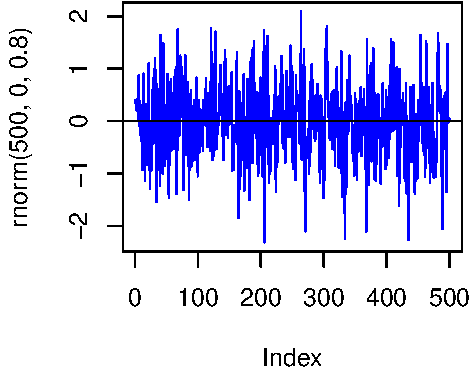
\includegraphics{FMC_T4_PhD_ARMA_GARCH_files/figure-latex/arima_sim-1} \end{center}

\begin{Shaded}
\begin{Highlighting}[]
\CommentTok{# AR(1)}
\NormalTok{ar_}\DecValTok{1}\NormalTok{ <-}\StringTok{ }\KeywordTok{arima.sim}\NormalTok{(}\DataTypeTok{n =} \DecValTok{500}\NormalTok{, }\KeywordTok{list}\NormalTok{(}\DataTypeTok{ar =} \KeywordTok{c}\NormalTok{(}\FloatTok{0.8}\NormalTok{)), }\DataTypeTok{sd =} \FloatTok{0.8}\NormalTok{)}
\KeywordTok{plot}\NormalTok{(ar_}\DecValTok{1}\NormalTok{, }\DataTypeTok{col =} \StringTok{"blue"}\NormalTok{)}
\KeywordTok{abline}\NormalTok{(}\DataTypeTok{h =} \DecValTok{0}\NormalTok{)}
\end{Highlighting}
\end{Shaded}

\begin{center}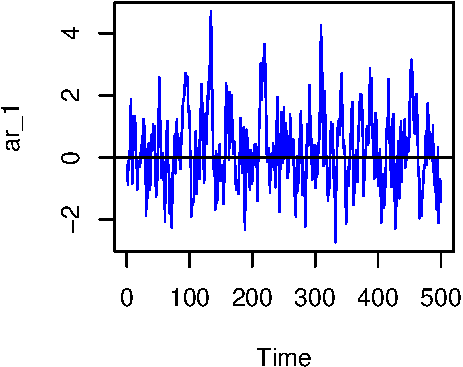
\includegraphics{FMC_T4_PhD_ARMA_GARCH_files/figure-latex/arima_sim-2} \end{center}

\begin{Shaded}
\begin{Highlighting}[]
\CommentTok{# AR(2)}
\NormalTok{ar_}\DecValTok{2}\NormalTok{ <-}\StringTok{ }\KeywordTok{arima.sim}\NormalTok{(}\DataTypeTok{n =} \DecValTok{500}\NormalTok{, }\KeywordTok{list}\NormalTok{(}\DataTypeTok{ar =} \KeywordTok{c}\NormalTok{(}\FloatTok{0.8}\NormalTok{, }\FloatTok{0.15}\NormalTok{)), }\DataTypeTok{sd =} \FloatTok{0.8}\NormalTok{)}
\KeywordTok{plot}\NormalTok{(ar_}\DecValTok{2}\NormalTok{, }\DataTypeTok{col =} \StringTok{"blue"}\NormalTok{)}
\KeywordTok{abline}\NormalTok{(}\DataTypeTok{h =} \DecValTok{0}\NormalTok{)}
\end{Highlighting}
\end{Shaded}

\begin{center}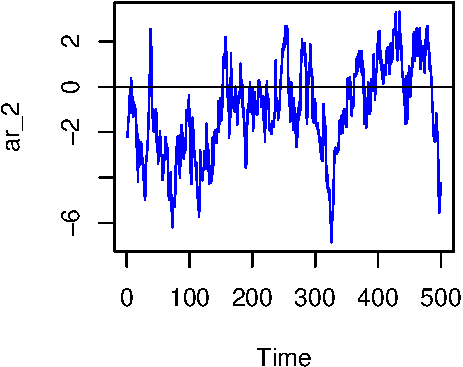
\includegraphics{FMC_T4_PhD_ARMA_GARCH_files/figure-latex/arima_sim-3} \end{center}

\begin{Shaded}
\begin{Highlighting}[]
\CommentTok{# AR(3)}
\NormalTok{ar_}\DecValTok{3}\NormalTok{ <-}\StringTok{ }\KeywordTok{arima.sim}\NormalTok{(}\DataTypeTok{n =} \DecValTok{500}\NormalTok{, }\KeywordTok{list}\NormalTok{(}\DataTypeTok{ar =} \KeywordTok{c}\NormalTok{(}\FloatTok{0.5}\NormalTok{, }\FloatTok{0.3}\NormalTok{, }\FloatTok{0.15}\NormalTok{)), }\DataTypeTok{sd =} \FloatTok{0.8}\NormalTok{)}
\KeywordTok{plot}\NormalTok{(ar_}\DecValTok{3}\NormalTok{, }\DataTypeTok{col =} \StringTok{"blue"}\NormalTok{)}
\KeywordTok{abline}\NormalTok{(}\DataTypeTok{h =} \DecValTok{0}\NormalTok{)}
\end{Highlighting}
\end{Shaded}

\begin{center}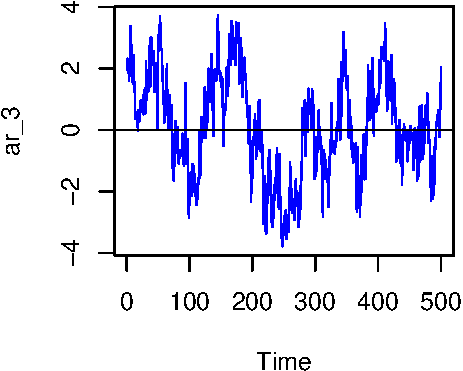
\includegraphics{FMC_T4_PhD_ARMA_GARCH_files/figure-latex/arima_sim-4} \end{center}

\subsubsection{Autocorrelation Function for AR(1)
processes}\label{autocorrelation-function-for-ar1-processes}

We can easily check that for positive lags \(l>0\), the lagged
covariance follows:

\[\gamma_l = \phi_1\gamma_{l-1}\]

Hence it follows that for the autocorrelation function
\(\rho_l = \phi_1\rho_{l-1}\); and becasue \(\rho_0=1\),
\(\rho_l = \phi_1^l\). This implies that the autocorrelation function of
an AR(1) series decays exponentially with rate \(\phi_1\) and starting
value 1. If \(\phi_1<0\) the series alternates between positive and
negative terms.

\textbf{Illustration}

For example let's compute the sample autocorrelation function (ACF) for
the financial market indices.

\begin{Shaded}
\begin{Highlighting}[]
\KeywordTok{acf}\NormalTok{(ret_BSE, }\DataTypeTok{na.action =}\NormalTok{ na.pass)}
\end{Highlighting}
\end{Shaded}

\begin{center}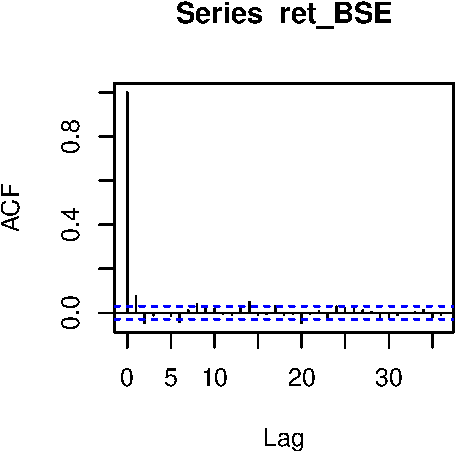
\includegraphics{FMC_T4_PhD_ARMA_GARCH_files/figure-latex/sample_ACF-1} \end{center}

\begin{Shaded}
\begin{Highlighting}[]
\KeywordTok{acf}\NormalTok{(ret_sp500, }\DataTypeTok{na.action =}\NormalTok{ na.pass)}
\end{Highlighting}
\end{Shaded}

\begin{center}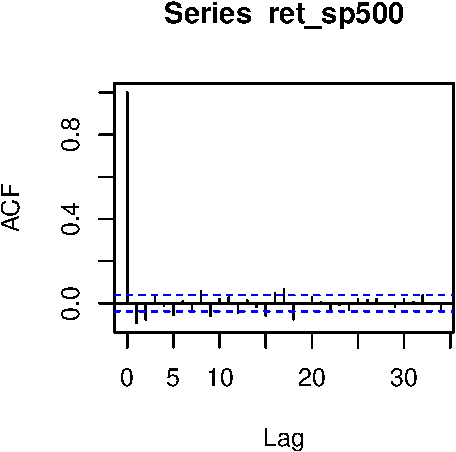
\includegraphics{FMC_T4_PhD_ARMA_GARCH_files/figure-latex/sample_ACF-2} \end{center}

\begin{Shaded}
\begin{Highlighting}[]
\KeywordTok{acf}\NormalTok{(ret_nikkei, }\DataTypeTok{na.action =}\NormalTok{ na.pass)}
\end{Highlighting}
\end{Shaded}

\begin{center}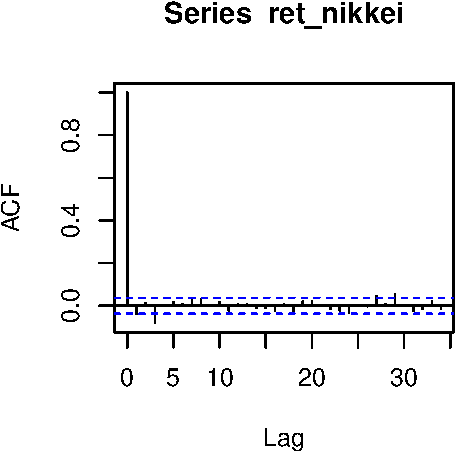
\includegraphics{FMC_T4_PhD_ARMA_GARCH_files/figure-latex/sample_ACF-3} \end{center}

What about log-returns?

\begin{Shaded}
\begin{Highlighting}[]
\NormalTok{logret_BSE <-}\StringTok{ }\KeywordTok{func_pr_to_logret}\NormalTok{(index_bse}\OperatorTok{$}\NormalTok{Close)}
\NormalTok{logret_SP <-}\StringTok{ }\KeywordTok{func_pr_to_logret}\NormalTok{(ind_sp500}\OperatorTok{$}\NormalTok{SP500)}
\NormalTok{logret_Nikkei <-}\StringTok{ }\KeywordTok{func_pr_to_logret}\NormalTok{(ind_nikkei}\OperatorTok{$}\NormalTok{NIKKEI225)}

\NormalTok{ACF_BSE <-}\StringTok{ }\KeywordTok{acf}\NormalTok{(logret_BSE, }\DataTypeTok{na.action =}\NormalTok{ na.pass)}
\end{Highlighting}
\end{Shaded}

\begin{center}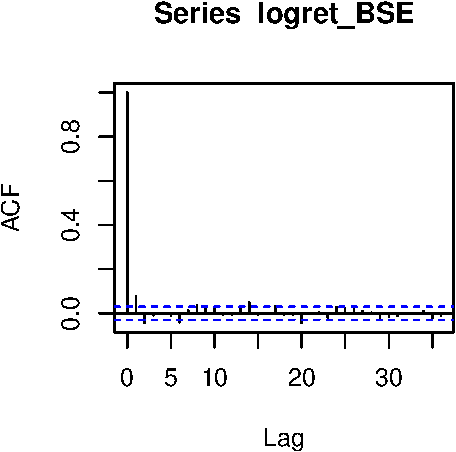
\includegraphics{FMC_T4_PhD_ARMA_GARCH_files/figure-latex/sample_ACF_logret-1} \end{center}

\begin{Shaded}
\begin{Highlighting}[]
\KeywordTok{barplot}\NormalTok{(}\KeywordTok{head}\NormalTok{(ACF_BSE}\OperatorTok{$}\NormalTok{acf))}
\end{Highlighting}
\end{Shaded}

\begin{center}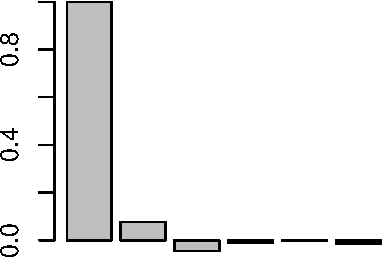
\includegraphics{FMC_T4_PhD_ARMA_GARCH_files/figure-latex/sample_ACF_logret-2} \end{center}

\begin{Shaded}
\begin{Highlighting}[]
\NormalTok{ACF_SP <-}\StringTok{ }\KeywordTok{acf}\NormalTok{(logret_SP, }\DataTypeTok{na.action =}\NormalTok{ na.pass)}
\end{Highlighting}
\end{Shaded}

\begin{center}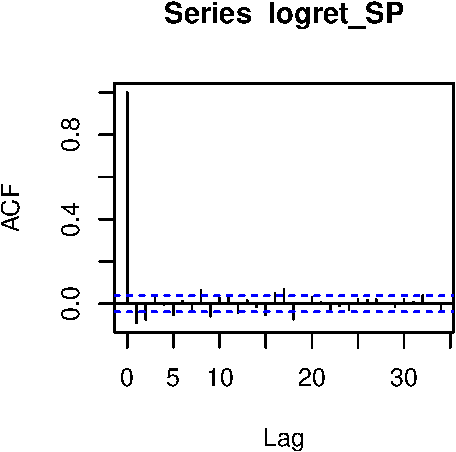
\includegraphics{FMC_T4_PhD_ARMA_GARCH_files/figure-latex/sample_ACF_logret-3} \end{center}

\begin{Shaded}
\begin{Highlighting}[]
\KeywordTok{barplot}\NormalTok{(}\KeywordTok{head}\NormalTok{(ACF_SP}\OperatorTok{$}\NormalTok{acf))}
\end{Highlighting}
\end{Shaded}

\begin{center}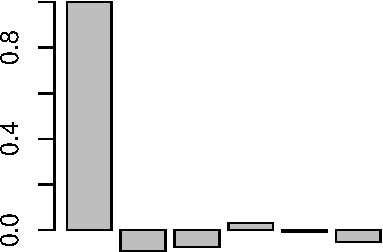
\includegraphics{FMC_T4_PhD_ARMA_GARCH_files/figure-latex/sample_ACF_logret-4} \end{center}

\begin{Shaded}
\begin{Highlighting}[]
\NormalTok{ACF_Nikkei <-}\StringTok{ }\KeywordTok{acf}\NormalTok{(logret_Nikkei, }\DataTypeTok{na.action =}\NormalTok{ na.pass)}
\end{Highlighting}
\end{Shaded}

\begin{center}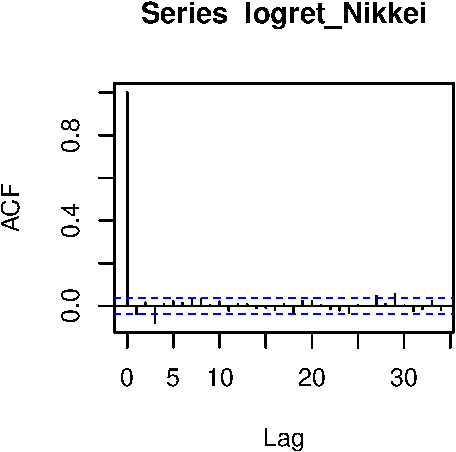
\includegraphics{FMC_T4_PhD_ARMA_GARCH_files/figure-latex/sample_ACF_logret-5} \end{center}

\begin{Shaded}
\begin{Highlighting}[]
\KeywordTok{barplot}\NormalTok{(}\KeywordTok{head}\NormalTok{(ACF_Nikkei}\OperatorTok{$}\NormalTok{acf))}
\end{Highlighting}
\end{Shaded}

\begin{center}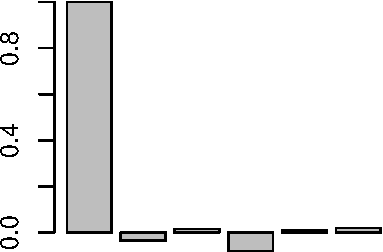
\includegraphics{FMC_T4_PhD_ARMA_GARCH_files/figure-latex/sample_ACF_logret-6} \end{center}

\subsubsection{Partial Autocorrelation Functions
(PACF)}\label{partial-autocorrelation-functions-pacf}

Is there a way to know how many lags to include for an autoregressive
return series? This issue is solved via the usage of \emph{partial
autocorrelation functions} as shown below.

Consider the following sequences of AR processes:

\[r_t=\phi_{01}+ \phi_{11}r_{t-1}+u_{1t}\]
\[r_t=\phi_{02}+ \phi_{12}r_{t-1}+\phi_{22}r_{t-2}+u_{2t}\]
\[r_t=\phi_{03}+ \phi_{13}r_{t-1}+\phi_{23}r_{t-2}+\phi_{33}r_{t-3}+u_{3t}\]
\[r_t=\phi_{04}+ \phi_{14}r_{t-1}+\phi_{24}r_{t-2}+\phi_{34}r_{t-3}+\phi_{44}r_{t-4}+u_{4t}\]
\[\vdots\]

These models are merely multiple regressions and can be estimated via
the standard least squares method.

In these models, \(\hat{\phi}_{11}\) is called the lag 1 sample PACF of
\(r_t\), \(\hat{\phi}_{22}\) of the second equation is the lag 2 sample
PACF of \(r_t\) and so on. By construction, the lag 2
\(\hat{\phi}_{22}\) is the marginal contribution of \(r_{t-2}\) in
explaining \(r_t\) over the AR(1) model and so on. Hence if the
underlying model is say AR(\(p\)) then all sample PACFs
\(\hat{\phi}_{11},\hdots, \hat{\phi}_{pp}\) must be different from 0 but
all sample PACFs from then on: \(\hat{\phi}_{p+1,p+1}, \hdots=0\). This
property can be used to find the order \(p\).

Armed with this knowledge, let's compute the PACFs for the three
financial market indices:

\begin{Shaded}
\begin{Highlighting}[]
\KeywordTok{pacf}\NormalTok{(ret_BSE, }\DataTypeTok{na.action =}\NormalTok{ na.pass)}
\end{Highlighting}
\end{Shaded}

\begin{center}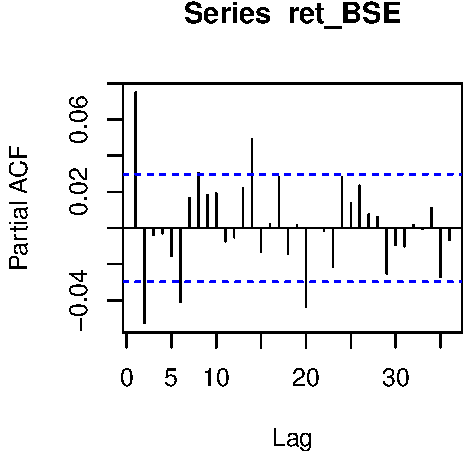
\includegraphics{FMC_T4_PhD_ARMA_GARCH_files/figure-latex/PACF-1} \end{center}

\begin{Shaded}
\begin{Highlighting}[]
\KeywordTok{pacf}\NormalTok{(ret_sp500, }\DataTypeTok{na.action =}\NormalTok{ na.pass)}
\end{Highlighting}
\end{Shaded}

\begin{center}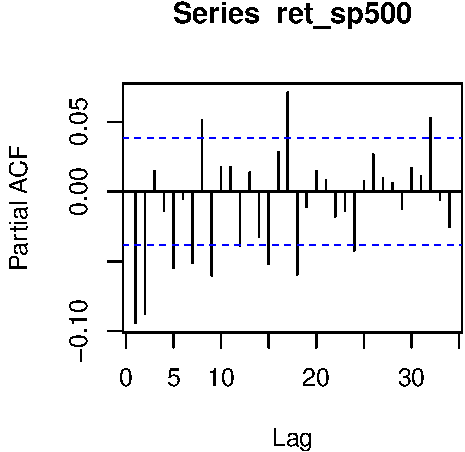
\includegraphics{FMC_T4_PhD_ARMA_GARCH_files/figure-latex/PACF-2} \end{center}

\begin{Shaded}
\begin{Highlighting}[]
\KeywordTok{pacf}\NormalTok{(ret_nikkei, }\DataTypeTok{na.action =}\NormalTok{ na.pass)}
\end{Highlighting}
\end{Shaded}

\begin{center}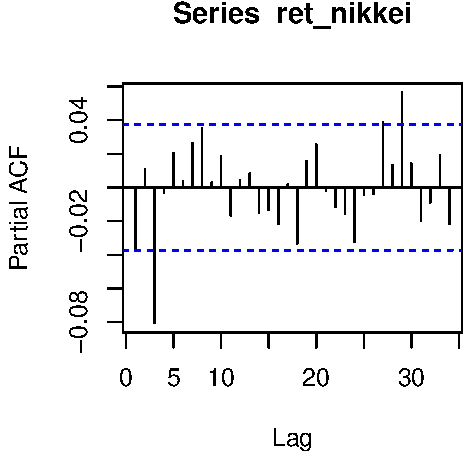
\includegraphics{FMC_T4_PhD_ARMA_GARCH_files/figure-latex/PACF-3} \end{center}

\subsubsection{Information Criteria}\label{information-criteria}

Apart from PACF, another way to find the number of lags is the use of
likelihood based information criteria. Here we look at the two most
famous ones: the Akaike Information Criterion (AIC) and the Bayesian
Information Criterion (BIC).

\[\text{AIC}(l) = -\frac{2}{T}\cdot\ln(\text{likelihood})+\frac{2}{T}\cdot(\#\text{parameters})\]

For a Gaussian AR(\(l\)),
\(AIC=\ln(\hat{\sigma}^2_{u,MLE})+2\frac{l}{T}\). The first term
measures the goodness of fit of the model while the second penalizes the
usage of parameters.

The Bayesian Information Criterion (BIC) uses a different penalty
function. For a Gaussian AR(\(l\)) is takes the following form:

\[BIC(l)=\ln(\hat{\sigma}^2_{u,MLE})+\ln(T)\cdot \frac{l}{T}\]

\section{Moving Average (MA)
Processes}\label{moving-average-ma-processes}

Consider an infinitely long autoregressive process:

\[r_t = \phi_0+\phi_1r_{t-1}+\phi_2r_{r-2}+\hdots+u_t\]

If this series is to be weakly stationary, the coefficients \(\phi_j\)
must decay sufficiently fast. One way to ensure this is to assume that
\(\phi_j=-\theta^j\) for some \(\theta\in(0,1)\).
\[r_t = \phi_0-\theta_1r_{t-1}-\theta_1^2r_{t-2}-\hdots+u_t\]
\[r_t+\sum_{j=1}^\infty \theta_1^jr_{t-j}=\phi_0+u_t\] The same form can
be written for \(r_{t-2}\):
\[r_{t-1}+\sum_{j=2}^\infty \theta_1^jr_{t-j}=\phi_0+u_{t-1}\]

Solving for the above two equations, we get:
\[r_t = \phi_0(1-\theta_1) + u_t -\theta_1u_{t-1}\]

This indicates the AR model is a weighted average of shocks
\(u_t, u_{t-1}\) and a constant. This is a \emph{moving average} form of
order 1 or MA(1). It's straightforward to check that unlike AR
processes, MA processes are \emph{always} stationary. (Can you see why?)

The general form for the MA(\(q\)) process is:
\[r_t = c_0 + u_t -\theta_1u_{t-1}-\theta_2u_{t-2}-\hdots-\theta_qu_{t-q}\]

\subsection{Autocorrelation Function}\label{autocorrelation-function}

Consider the MA(1) model with the constant term 0:

\[r_{t} = u_t -\theta_1u_{t-1}\]
\[r_{t-l}r_t = u_tr_{t-l} -\theta_1u_{t-1}r_{t-l}\]
\[\mathbb{E}(r_{t-l}r_t)=0-\theta_1\mathbb{E}(u_{t-1}r_{t-l})\] From
this we see that: \[\gamma_1=-\theta_1\sigma^2_u\] \[\gamma_{l>1}=0\]
Also, \(\text{var}(r_t) =\gamma_0= (1+\theta_1^2)\sigma_u^2\) and this
implies that for \(\rho_l = \frac{\gamma_l}{\gamma_0}\) becomes:
\[\rho_0 = 1\] \[\rho_1 = -\frac{\theta_1}{1+\theta_1^2}\]
\[\rho_{l>1} = 0\]

Hence for MA(1) processes, while the first lag autocorrelation is
nonzero, all further lags produce zero autocorrelation. This property
can be exploited to locate the order of the MA process. In general, for
an MA(\(q\)) process, the ACF cuts off at lag \(q\). Since the MA(\(q\))
process only relies on its past \(q-1\) realization, it's often called a
`finite memory' process.

To check the order of the MA series in question, we plot the ACF of the
series. If \(\rho_q\neq 0\) but \(\rho_{l>q}=0\) we may conclude that
the series is MA(\(q\)).

\subsubsection{Illustrations}\label{illustrations}

We simulate some moving average processes below:

\begin{Shaded}
\begin{Highlighting}[]
\NormalTok{n <-}\StringTok{ }\DecValTok{500}

\CommentTok{# MA(0)}
\KeywordTok{plot}\NormalTok{(}\KeywordTok{rnorm}\NormalTok{(n), }\DataTypeTok{type =} \StringTok{"l"}\NormalTok{, }\DataTypeTok{col =} \StringTok{"blue"}\NormalTok{)}
\KeywordTok{abline}\NormalTok{(}\DataTypeTok{h =} \DecValTok{0}\NormalTok{)}
\end{Highlighting}
\end{Shaded}

\begin{center}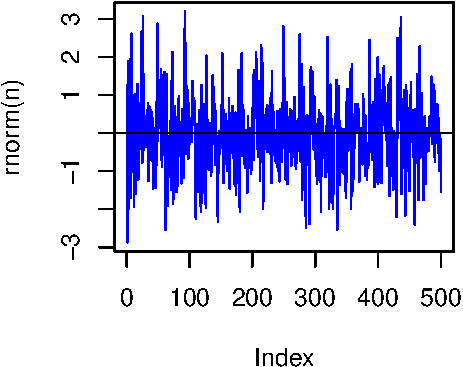
\includegraphics{FMC_T4_PhD_ARMA_GARCH_files/figure-latex/MA-1} \end{center}

\begin{Shaded}
\begin{Highlighting}[]
\CommentTok{# MA(1)}
\NormalTok{ma_}\DecValTok{1}\NormalTok{ <-}\StringTok{ }\KeywordTok{arima.sim}\NormalTok{(}\DataTypeTok{n =}\NormalTok{ n, }\KeywordTok{list}\NormalTok{(}\DataTypeTok{ma =} \KeywordTok{c}\NormalTok{(}\FloatTok{0.8}\NormalTok{)), }\DataTypeTok{innov=}\KeywordTok{rnorm}\NormalTok{(n))}
\KeywordTok{plot}\NormalTok{(ma_}\DecValTok{1}\NormalTok{, }\DataTypeTok{col =} \StringTok{"blue"}\NormalTok{)}
\KeywordTok{abline}\NormalTok{(}\DataTypeTok{h =} \DecValTok{0}\NormalTok{)}
\end{Highlighting}
\end{Shaded}

\begin{center}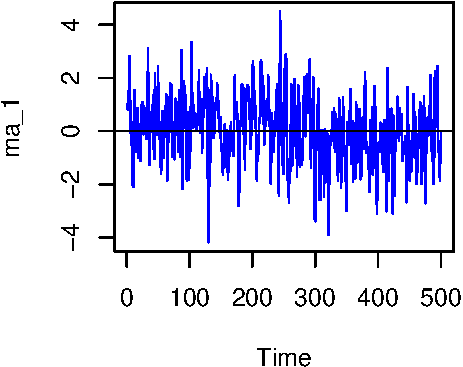
\includegraphics{FMC_T4_PhD_ARMA_GARCH_files/figure-latex/MA-2} \end{center}

\begin{Shaded}
\begin{Highlighting}[]
\CommentTok{# MA(2)}
\NormalTok{ma_}\DecValTok{2}\NormalTok{ <-}\StringTok{ }\KeywordTok{arima.sim}\NormalTok{(}\DataTypeTok{n =}\NormalTok{ n, }\KeywordTok{list}\NormalTok{(}\DataTypeTok{ma =} \KeywordTok{c}\NormalTok{(}\FloatTok{0.8}\NormalTok{, }\FloatTok{0.15}\NormalTok{)), }\DataTypeTok{innov=}\KeywordTok{rnorm}\NormalTok{(n))}
\KeywordTok{plot}\NormalTok{(ma_}\DecValTok{2}\NormalTok{, }\DataTypeTok{col =} \StringTok{"blue"}\NormalTok{)}
\KeywordTok{abline}\NormalTok{(}\DataTypeTok{h =} \DecValTok{0}\NormalTok{)}
\end{Highlighting}
\end{Shaded}

\begin{center}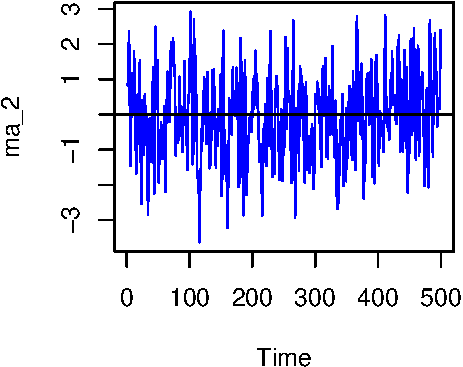
\includegraphics{FMC_T4_PhD_ARMA_GARCH_files/figure-latex/MA-3} \end{center}

\begin{Shaded}
\begin{Highlighting}[]
\CommentTok{# MA(3)}
\NormalTok{ma_}\DecValTok{3}\NormalTok{ <-}\StringTok{ }\KeywordTok{arima.sim}\NormalTok{(}\DataTypeTok{n =}\NormalTok{ n, }\KeywordTok{list}\NormalTok{(}\DataTypeTok{ma =} \KeywordTok{c}\NormalTok{(}\FloatTok{0.5}\NormalTok{, }\FloatTok{0.3}\NormalTok{, }\FloatTok{0.15}\NormalTok{)), }\DataTypeTok{innov=}\KeywordTok{rnorm}\NormalTok{(n))}
\KeywordTok{plot}\NormalTok{(ma_}\DecValTok{3}\NormalTok{, }\DataTypeTok{col =} \StringTok{"blue"}\NormalTok{)}
\KeywordTok{abline}\NormalTok{(}\DataTypeTok{h =} \DecValTok{0}\NormalTok{)}
\end{Highlighting}
\end{Shaded}

\begin{center}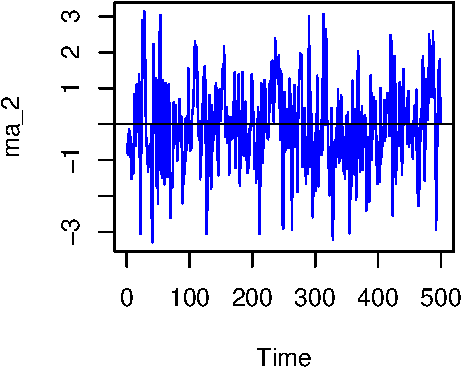
\includegraphics{FMC_T4_PhD_ARMA_GARCH_files/figure-latex/MA-4} \end{center}

\section{Autoregressive Moving Average (ARMA)
Processes}\label{autoregressive-moving-average-arma-processes}

While in principle we could fit empirical time series to AR(\(p\)) or
MA(\(q\)) models exclusively, often the concomitant order is very high.
In order to circumevent this problem, we combine AR and MA models into a
composite ARMA(\(p,q\)) model with fewer parameters to estimate.

For example the ARMA(1,1) series is as follows:
\[r_t-\phi_1r_{t-1} = \phi_0 + u_t -\theta_1u_{t-1}\]

The LHS is the AR component while the RHS is MA component.

\subsection{Properties}\label{properties}

Taking expectations we get:
\[\mathbb{E}(r_t)-\phi_1\mathbb{E}(r_{t-1}) = \phi_0 + \mathbb{E}(u_t) - \theta_1\mathbb{E}(u_{t-1})\]
\[\mathbb{E}(r_t) = \mu = \frac{\phi_0}{1-\phi_1}\]

This is the same exact mean as that of an AR(1) process. Solving for the
stationarity of the variance we get the same condition for the parameter
\(\phi_1\in (0,1)\) as that of the AR(1) model. It is not hard to derive
the autocorrelation function of the ARMA(1,1) process which behaves the
same way as that of an AR(1) process.

In general for an ARMA(\(p, q\)) process we have the following
definition:

\[r_t = \phi_0 + \sum_{i=1}^p \phi_ir_{t-i}+u_t-\sum_{j=1}^q \theta_ju_{t-j}\]

\section{Conditional Heteroskedasticity
Models}\label{conditional-heteroskedasticity-models}

In empirical time series, we do not observe volatility directly but only
estimate it with the help of some other directly observed
characteristics. However as discussed in Cont (2001) volatility displays
some striking regularities such as volatility clustering and
differential reaction to price changes.

To investigate the volatility of empirical time series, we plot the
daily returns and ACF of the Bombay stock exchange sensex.

\begin{Shaded}
\begin{Highlighting}[]
\KeywordTok{plot}\NormalTok{(logret_BSE, }\DataTypeTok{type =} \StringTok{"l"}\NormalTok{, }\DataTypeTok{col =} \StringTok{"blue"}\NormalTok{)}
\KeywordTok{abline}\NormalTok{(}\DataTypeTok{h =} \DecValTok{0}\NormalTok{)}
\end{Highlighting}
\end{Shaded}

\begin{center}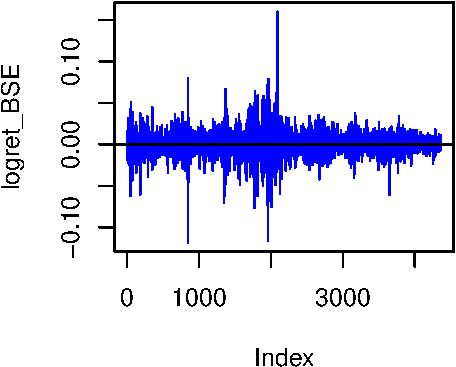
\includegraphics{FMC_T4_PhD_ARMA_GARCH_files/figure-latex/BSE_ret_ACF-1} \end{center}

\begin{Shaded}
\begin{Highlighting}[]
\KeywordTok{plot}\NormalTok{(}\KeywordTok{acf}\NormalTok{(ret_BSE, }\DataTypeTok{na.action =}\NormalTok{ na.pass))}
\end{Highlighting}
\end{Shaded}

\begin{center}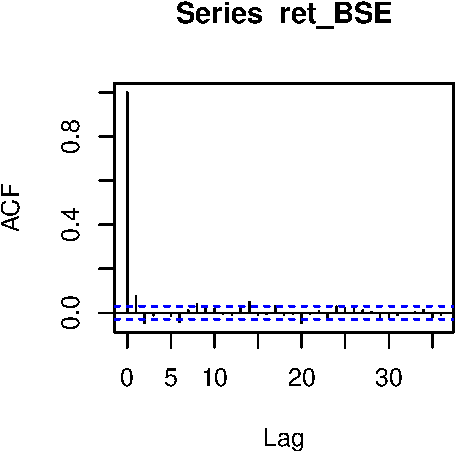
\includegraphics{FMC_T4_PhD_ARMA_GARCH_files/figure-latex/BSE_ret_ACF-2} \end{center}

While there seems to be no serial autocorrelation there is some
dependence structure embedded in the series. We can check this for
various functions of the return process such as squared returns or
absolute returns:

\begin{Shaded}
\begin{Highlighting}[]
\NormalTok{ret_BSE_sq <-}\StringTok{ }\NormalTok{ret_BSE}\OperatorTok{^}\DecValTok{2}
\KeywordTok{acf}\NormalTok{(ret_BSE_sq, }\DataTypeTok{na.action =}\NormalTok{ na.pass)}
\end{Highlighting}
\end{Shaded}

\begin{center}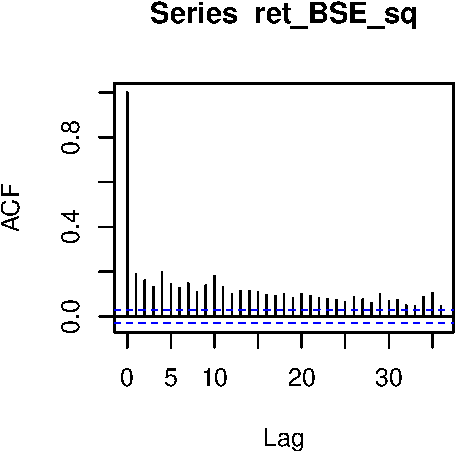
\includegraphics{FMC_T4_PhD_ARMA_GARCH_files/figure-latex/BSE_ret_ACF_sq-1} \end{center}

\begin{Shaded}
\begin{Highlighting}[]
\KeywordTok{pacf}\NormalTok{(ret_BSE_sq, }\DataTypeTok{na.action =}\NormalTok{ na.pass)}
\end{Highlighting}
\end{Shaded}

\begin{center}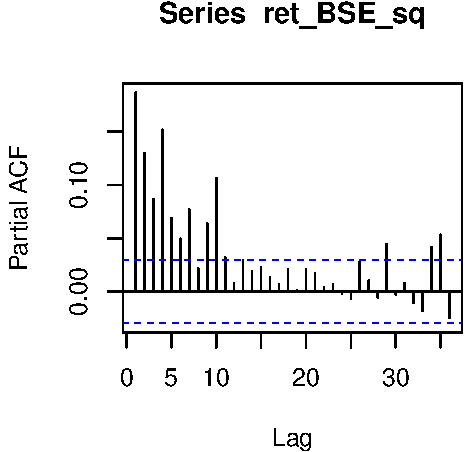
\includegraphics{FMC_T4_PhD_ARMA_GARCH_files/figure-latex/BSE_ret_ACF_sq-2} \end{center}

\begin{Shaded}
\begin{Highlighting}[]
\NormalTok{ret_BSE_abs <-}\StringTok{ }\KeywordTok{abs}\NormalTok{(ret_BSE)}
\KeywordTok{acf}\NormalTok{(ret_BSE_abs, }\DataTypeTok{na.action =}\NormalTok{ na.pass)}
\end{Highlighting}
\end{Shaded}

\begin{center}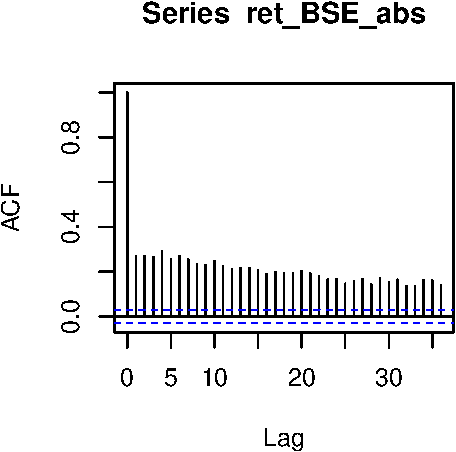
\includegraphics{FMC_T4_PhD_ARMA_GARCH_files/figure-latex/BSE_ret_ACF_sq-3} \end{center}

\begin{Shaded}
\begin{Highlighting}[]
\KeywordTok{pacf}\NormalTok{(ret_BSE_abs, }\DataTypeTok{na.action =}\NormalTok{ na.pass)}
\end{Highlighting}
\end{Shaded}

\begin{center}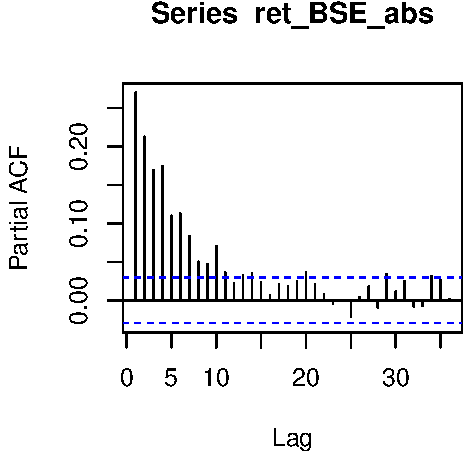
\includegraphics{FMC_T4_PhD_ARMA_GARCH_files/figure-latex/BSE_ret_ACF_sq-4} \end{center}

This behavior is also displayed by the other financial markets.

\begin{Shaded}
\begin{Highlighting}[]
\KeywordTok{acf}\NormalTok{(ret_sp500}\OperatorTok{^}\DecValTok{2}\NormalTok{, }\DataTypeTok{na.action =}\NormalTok{ na.pass)}
\end{Highlighting}
\end{Shaded}

\begin{center}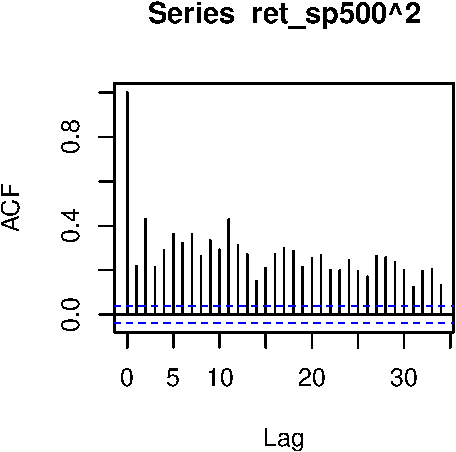
\includegraphics{FMC_T4_PhD_ARMA_GARCH_files/figure-latex/ret_ind_ACF_sq-1} \end{center}

\begin{Shaded}
\begin{Highlighting}[]
\KeywordTok{pacf}\NormalTok{(ret_sp500}\OperatorTok{^}\DecValTok{2}\NormalTok{, }\DataTypeTok{na.action =}\NormalTok{ na.pass)}
\end{Highlighting}
\end{Shaded}

\begin{center}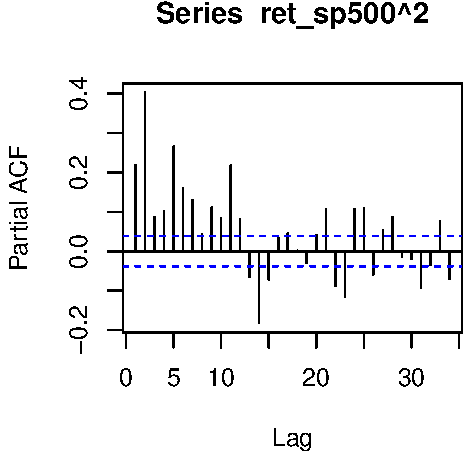
\includegraphics{FMC_T4_PhD_ARMA_GARCH_files/figure-latex/ret_ind_ACF_sq-2} \end{center}

\begin{Shaded}
\begin{Highlighting}[]
\KeywordTok{acf}\NormalTok{(ret_nikkei}\OperatorTok{^}\DecValTok{2}\NormalTok{, }\DataTypeTok{na.action =}\NormalTok{ na.pass)}
\end{Highlighting}
\end{Shaded}

\begin{center}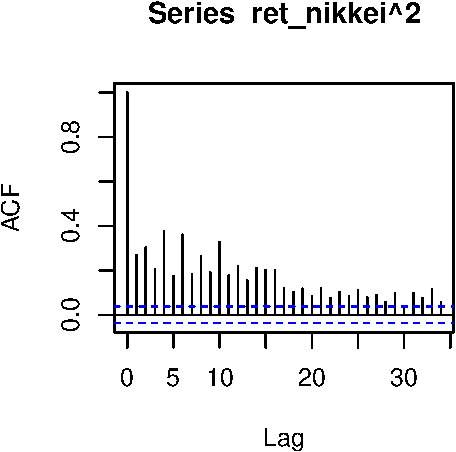
\includegraphics{FMC_T4_PhD_ARMA_GARCH_files/figure-latex/ret_ind_ACF_sq-3} \end{center}

\begin{Shaded}
\begin{Highlighting}[]
\KeywordTok{pacf}\NormalTok{(ret_nikkei}\OperatorTok{^}\DecValTok{2}\NormalTok{, }\DataTypeTok{na.action =}\NormalTok{ na.pass)}
\end{Highlighting}
\end{Shaded}

\begin{center}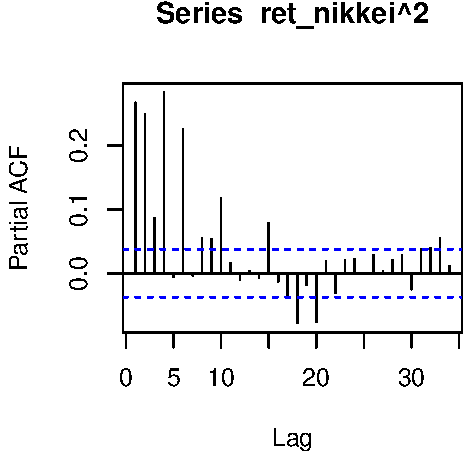
\includegraphics{FMC_T4_PhD_ARMA_GARCH_files/figure-latex/ret_ind_ACF_sq-4} \end{center}

The conditional mean volatility of the series may be written as:

\[\mu_t = \mathbb{E}(r_t|\mathbb{F}_{t-1})\]
\[\sigma_t^2 = \text{var}(r_t|\mathbb{F}_{t-1}) = \mathbb{E}((r_t-\mu_t)^2|\mathbb{F}_{t-1})
=\text{var}(u_t|\mathbb{F}_{t-1})\]

Here \(\mathbb{F}(\cdot)\) denotes the `filtration' or the information
available at the given time.

\subsection{ARCH Effect}\label{arch-effect}

Consider \(r_t = \mu_t + u_t\). The square of the residual series
\(u_t = r_t - \mu_t\) is of interest for estimating conditional
heteroskedasticity, also known as the ARCH effect (autoregressive
conditional heteroskedasticity effect). A popular method of testing for
ARCH effects is via Engel's Lagrange multiplier test which is equivalent
to the standard \(F\) statistic for testing \(\beta_i=0\) in the
multiple linear regression:

\[u_t^2 = \beta_0 + \beta_1u_{t-1}^2 + \hdots + \beta_m u_{t-m}^2 + \epsilon_t \]

\section*{References}\label{references}
\addcontentsline{toc}{section}{References}

\hypertarget{refs}{}
\hypertarget{ref-Cont:2001}{}
Cont, Rama. 2001. ``Empirical Properties of Asset Returns: Stylized
Facts and Statistical Issues.'' \emph{Quantitative Finance} 1 (2):
223--36.

\hypertarget{ref-Jondeau_Poon_Rockinger:2007}{}
Jondeau, Eric, Ser-Huang Poon, and Michael Rockinger. 2007.
\emph{Financial Modeling Under Non-Gaussian Distributions}. Springer
Finance.

\hypertarget{ref-Tsay:2010}{}
Tsay, Ruey S. 2010. \emph{Analysis of Financial Time Series}. Third
Edition. John Wiley; Sons.


\end{document}
